\chapter{De las materias primas al reciclaje}\label{ch:g5:raw-materials-and-recycling}

Una lata de refresco vacía cae en un contenedor de \omterm{def:g5:raw-materials-and-recycling:recycling}{reciclaje}. Un camión
la lleva a una planta de clasificación, una máquina la aplasta junto con
miles de otras hasta formar un bloque, un horno funde los bloques y,
unas semanas después, el metal vuelve a estar en la estantería de una
tienda convertido en una lata nueva. ¿De dónde salió el metal al
principio, y por qué merece la pena fundir latas viejas en lugar de
fabricar metal nuevo?

\begin{recall}
Un objeto es una cosa que podemos ver y tocar; su material es aquello de
lo que está hecho: madera, metal, vidrio, plástico, papel, tela, piedra
(\cref{ch:g1:materials-around-us}). En un \omterm{def:g5:irreversible-changes:chemical-change}{cambio químico} aparecen
sustancias nuevas y no hay un camino de vuelta sencillo (\cref{ch:g5:irreversible-changes}).
\end{recall}

\section{Materiales naturales y elaborados}

\begin{definition}[Materiales naturales y elaborados]\label{def:g5:raw-materials-and-recycling:natural-material}
Un \emph{material natural}\index{material natural} se usa casi tal como
se encuentra en la naturaleza, solo cortado o moldeado: la madera, la
piedra, el algodón, la lana, el cuero.
Un \emph{material elaborado}\index{material elaborado} lo fabrican
las personas a partir de sustancias que se encuentran en la naturaleza,
transformándolas, a menudo con calor y con \omterm{def:g5:irreversible-changes:chemical-change}{cambios químicos}: el vidrio,
el acero, el aluminio, el plástico, el papel, el hormigón.
\end{definition}

\begin{example}[Dos mesas]\label{ex:g5:raw-materials-and-recycling:tables}
Una mesa hecha con tablas de roble es de un \omterm{def:g5:raw-materials-and-recycling:natural-material}{material natural}: la madera
solo se ha serrado, cepillado y encolado. Una mesa con tablero de vidrio
y patas de acero es de \omterm{def:g5:raw-materials-and-recycling:natural-material}{materiales elaborados}: ni el vidrio ni el acero
se encuentran tal cual en la naturaleza.
\end{example}

\section{Las materias primas}

\begin{definition}[Materia prima y mena]\label{def:g5:raw-materials-and-recycling:raw-material}
Una \emph{materia prima}\index{materia prima} es una sustancia que se
toma de la naturaleza para fabricar materiales y objetos: los árboles,
la arena, las rocas, el petróleo, el algodón, la lana. Una roca de la
que se extrae un metal se llama
\emph{mena}\index{mena}.
\end{definition}

\begin{example}[De dónde vienen los materiales]\label{ex:g5:raw-materials-and-recycling:from}
\begin{itemize}
  \item la madera y el papel vienen de los árboles;
  \item el vidrio viene de la arena, calentada muy fuerte con sosa y
        caliza;
  \item el hierro y el acero vienen de la \omterm{def:g5:raw-materials-and-recycling:raw-material}{mena} de hierro, una roca
        rojiza;
  \item el aluminio viene de la bauxita, otra \omterm{def:g5:raw-materials-and-recycling:raw-material}{mena};
  \item casi todos los plásticos vienen del petróleo, que se bombea del
        subsuelo;
  \item el algodón viene de una planta, y la lana, de las ovejas.
\end{itemize}
\end{example}

\begin{omfigure}
\begin{minipage}[b]{0.48\linewidth}\centering
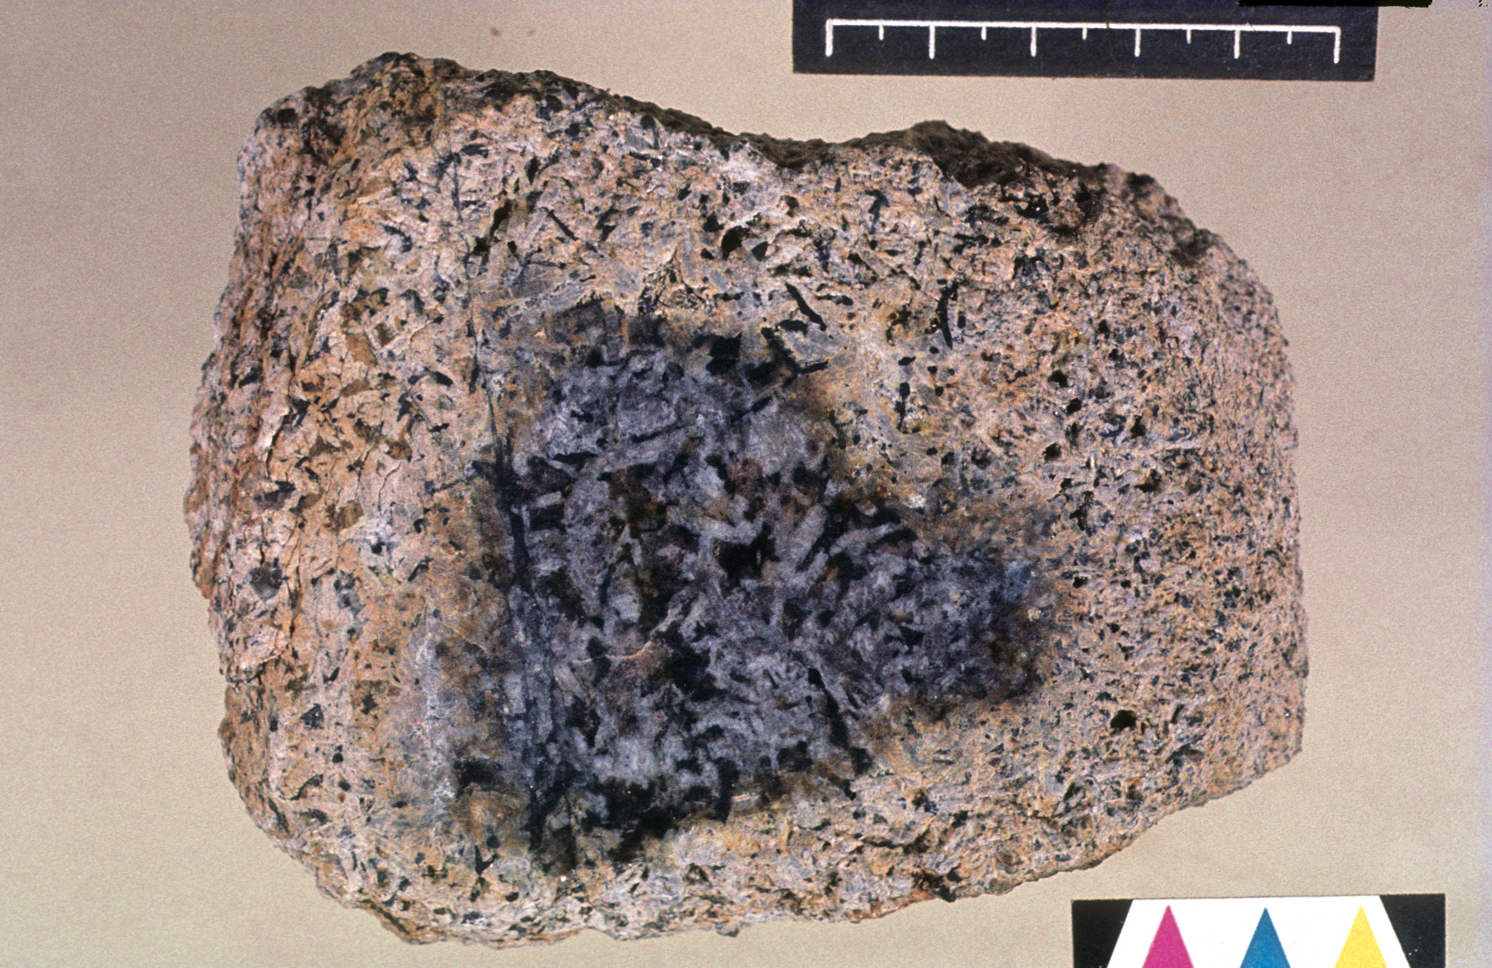
\includegraphics[width=\linewidth,height=4.6cm,keepaspectratio]{images/book1/bauxite.jpg}

{\small Bauxita, la \omterm{def:g5:raw-materials-and-recycling:raw-material}{mena} del aluminio, alrededor de un núcleo de roca
sin alterar. Foto: Werner Schellmann, CC BY-SA 2.5.}
\end{minipage}\hfill
\begin{minipage}[b]{0.48\linewidth}\centering
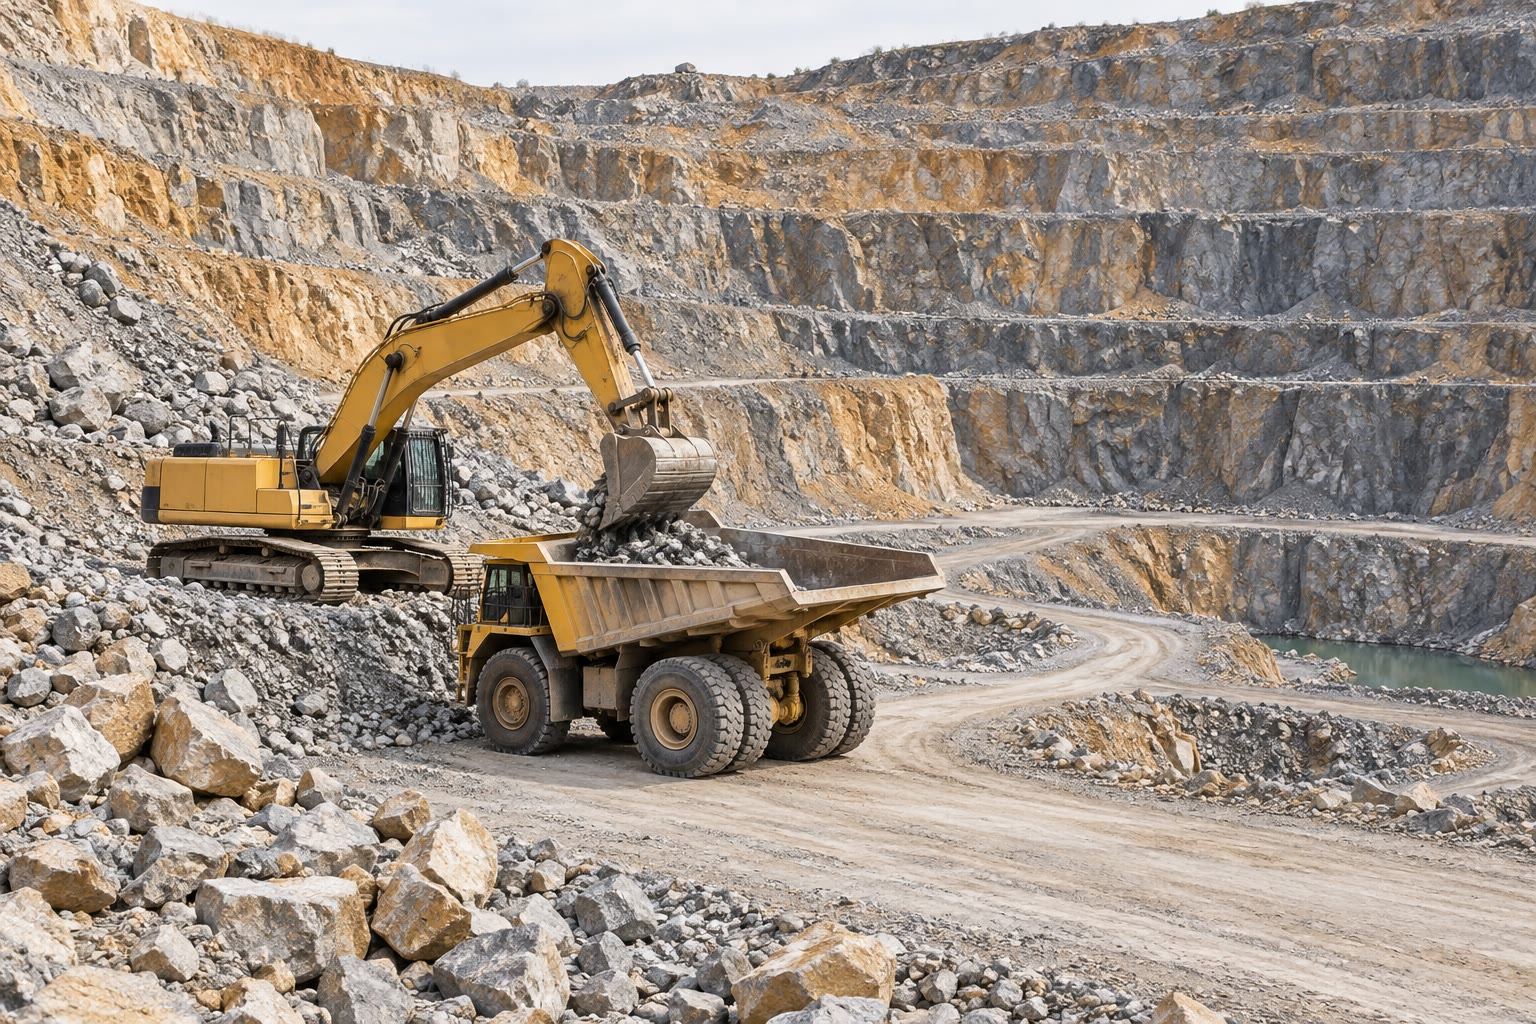
\includegraphics[width=\linewidth,height=4.6cm,keepaspectratio]{images/book1/ai/g5-quarry.jpg}

{\small Una cantera: se extrae la roca para usarla como \omterm{def:g5:raw-materials-and-recycling:raw-material}{materia prima}.}
\end{minipage}
\end{omfigure}

\begin{omfigure}
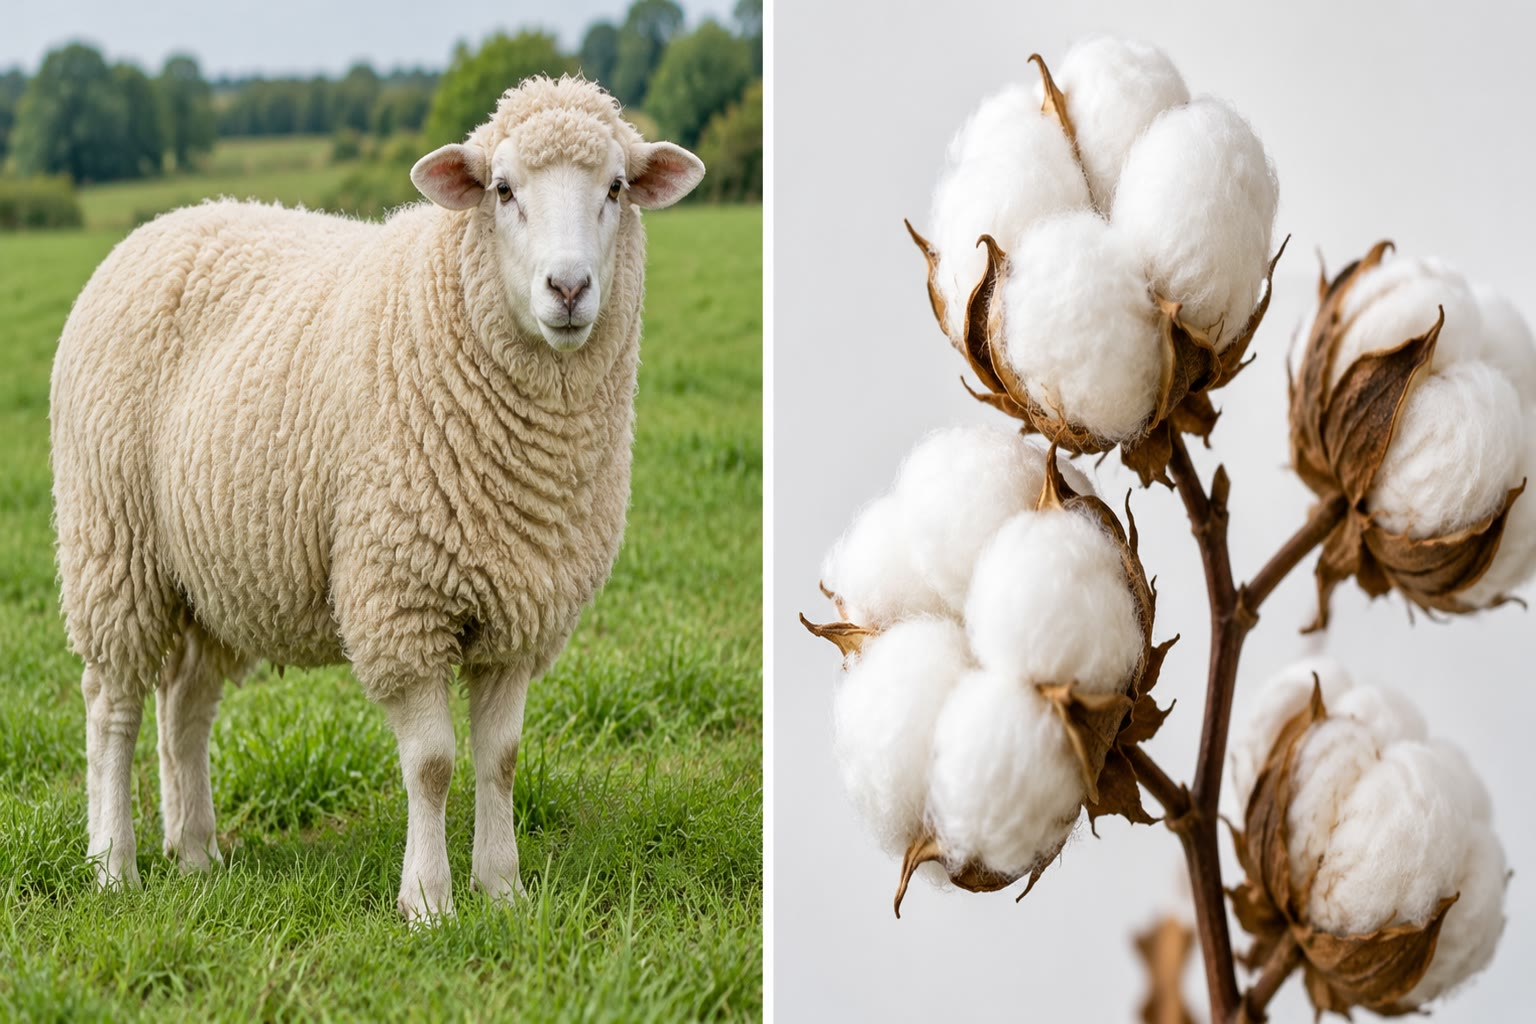
\includegraphics[width=0.6\linewidth]{images/book1/ai/g5-sheep-cotton.jpg}

{\small \omterm{def:g5:raw-materials-and-recycling:raw-material}{Materias primas} naturales que vienen de seres vivos: la lana de
las ovejas y el algodón de la planta del algodón.}
\end{omfigure}

\section{De la materia prima al objeto}

\begin{proposition}[Fabricar un material transforma su materia prima]\label{prop:g5:raw-materials-and-recycling:change}
Convertir una \omterm{def:g5:raw-materials-and-recycling:raw-material}{materia prima} en un \omterm{def:g5:raw-materials-and-recycling:natural-material}{material elaborado} requiere energía
(casi siempre el calor de un horno) y, por lo general, \omterm{def:g5:irreversible-changes:chemical-change}{cambios
químicos}: la arena se convierte en vidrio, la \omterm{def:g5:raw-materials-and-recycling:raw-material}{mena} en metal, el
petróleo en plástico. Estos cambios no se pueden deshacer sin más: el
vidrio no vuelve a ser arena.
\end{proposition}

\begin{example}[La vida de una botella de vidrio]\label{ex:g5:raw-materials-and-recycling:bottle}
Se calientan juntas en un horno arena, sosa y caliza triturada hasta que
se funden y forman vidrio. El vidrio caliente se sopla para darle forma
de botella. La botella se llena, se vende y se vacía. Si se tira al
contenedor de vidrio, se tritura en trocitos, se vuelve a fundir y se
sopla para hacer una botella nueva: el vidrio se usa una y otra vez.
\end{example}

\begin{omfigure}
\begin{tikzpicture}[font=\small,
    box/.style={draw=omDef, fill=omDef!6, rounded corners=2pt, align=center,
      minimum height=0.95cm, text width=2.4cm}]
  \node[box] (r) at (0,2.6) {materia prima\\ (arena, mena, petróleo)};
  \node[box] (m) at (4.0,2.6) {fabricación\\ del material};
  \node[box] (o) at (8.0,2.6) {objeto,\\ usado};
  \node[box] (w) at (8.0,0) {residuo};
  \node[box, draw=omProp, fill=omProp!8] (s) at (4.0,0) {clasificación\\ y reciclaje};
  \draw[->, thick, omDef] (r) -- (m);
  \draw[->, thick, omDef] (m) -- (o);
  \draw[->, thick, omDef] (o) -- (w);
  \draw[->, thick, omProp] (w) -- (s);
  \draw[->, thick, omProp] (s) -- (m) node[midway, left, align=right, text=black]
    {se usa de nuevo\\ en lugar de\\ materia prima nueva};
  \draw[->, thick, black!45, dashed] (w.east) -- ++(1.4,0) node[right, align=left,
    text=black] {se tira:\\ vertedero};
\end{tikzpicture}

{\small La vida de un material. El bucle naranja es el \omterm{def:g5:raw-materials-and-recycling:recycling}{reciclaje}: el
material de un objeto viejo sustituye a \omterm{def:g5:raw-materials-and-recycling:raw-material}{materia prima} nueva.}
\end{omfigure}

\section{Clasificar y reciclar}

\begin{definition}[Reciclaje]\label{def:g5:raw-materials-and-recycling:recycling}
El \emph{reciclaje}\index{reciclaje} consiste en recoger los objetos
usados y tratar su material para fabricar con él objetos nuevos, en
lugar de tirarlo.
\end{definition}

\begin{proposition}[Por qué reciclar]\label{prop:g5:raw-materials-and-recycling:why}
% ledger: al:energy-primary, al:energy-recycled (8.3 / 186 = about 1/22)
El \omterm{def:g5:raw-materials-and-recycling:recycling}{reciclaje} ahorra \omterm{def:g5:raw-materials-and-recycling:raw-material}{materias primas}, que así no hay que extraer del
subsuelo, y a menudo ahorra energía. Fabricar aluminio a partir de latas
viejas requiere solo una veinteava parte, más o menos, de la energía
necesaria para fabricarlo a partir de bauxita. Además, supone menos
residuos en los vertederos.
\end{proposition}

\begin{method}[Separar los residuos para reciclarlos]\label{met:g5:raw-materials-and-recycling:sort}
El \omterm{def:g5:raw-materials-and-recycling:recycling}{reciclaje} empieza por separar los residuos, allí donde se tiran:
\begin{enumerate}
  \item las botellas y los tarros de vidrio, en un contenedor;
  \item las latas de metal, el papel y el cartón y las botellas de
        plástico, en los contenedores que el municipio pone para ellos
        (los colores de los contenedores cambian de un sitio a otro);
  \item lo que no se puede reciclar, con el resto de los residuos.
\end{enumerate}
Cada material se recicla a su manera, así que un contenedor solo debe
contener los materiales a los que está destinado.
\end{method}

\begin{omfigure}
\begin{tikzpicture}[font=\small]
  \foreach \k/\t/\bc in {0/vidrio/green!50!black, 1/{latas de metal}/gray,
                        2/{papel y cartón}/omDef, 3/{botellas de plástico}/orange!80!black} {
    \begin{scope}[xshift=\k*3.4cm]
      \fill[\bc!18, draw=\bc, line width=0.8pt] (-1,0) -- (1,0) -- (1.15,2.0)
        -- (-1.15,2.0) -- cycle;
      \fill[\bc!45, draw=\bc] (-1.25,2.0) rectangle (1.25,2.3);
      \node[anchor=north, align=center] at (0,-0.15) {\t};
    \end{scope}
  }
  % glass: a bottle
  \fill[green!40!black!60] (-0.2,0.3) rectangle (0.2,1.2);
  \fill[green!40!black!60] (-0.07,1.2) rectangle (0.07,1.6);
  % metal: a can
  \begin{scope}[xshift=3.4cm]
    \fill[black!25, draw=black!55] (-0.3,0.3) rectangle (0.3,1.3);
  \end{scope}
  % paper: a box and a sheet
  \begin{scope}[xshift=6.8cm]
    \fill[brown!25, draw=brown!60] (-0.6,0.3) rectangle (0.1,1.0);
    \fill[white, draw=black!40] (0.2,0.3) rectangle (0.65,1.3);
  \end{scope}
  % plastic: a bottle
  \begin{scope}[xshift=10.2cm]
    \fill[cyan!20, draw=cyan!50!black] (-0.25,0.3) rectangle (0.25,1.3);
    \fill[cyan!20, draw=cyan!50!black] (-0.1,1.3) rectangle (0.1,1.6);
  \end{scope}
\end{tikzpicture}

{\small Cuatro contenedores, uno por material. (Los colores de los
contenedores reales cambian de una ciudad a otra.)}
\end{omfigure}

\begin{omfigure}
\begin{minipage}[t]{0.48\linewidth}\centering
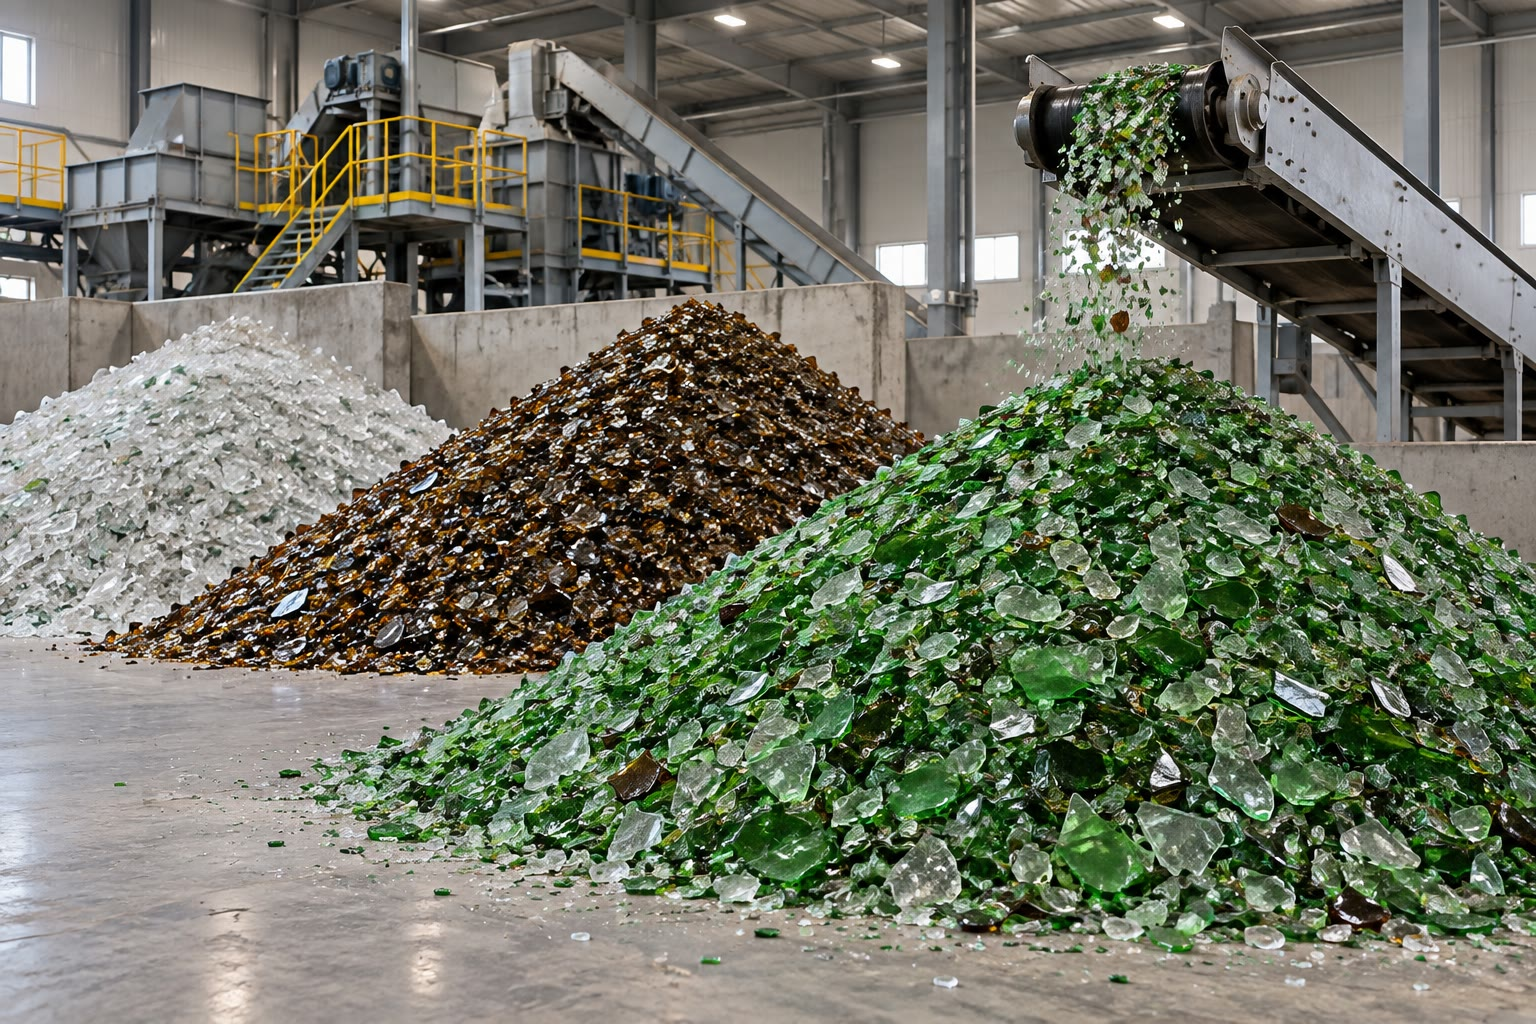
\includegraphics[width=\linewidth,height=4.6cm,keepaspectratio]{images/book1/ai/g5-glass-cullet.jpg}

{\small Vidrio triturado en una planta de \omterm{def:g5:raw-materials-and-recycling:recycling}{reciclaje}, listo para fundirse.}
\end{minipage}\hfill
\begin{minipage}[t]{0.48\linewidth}\centering
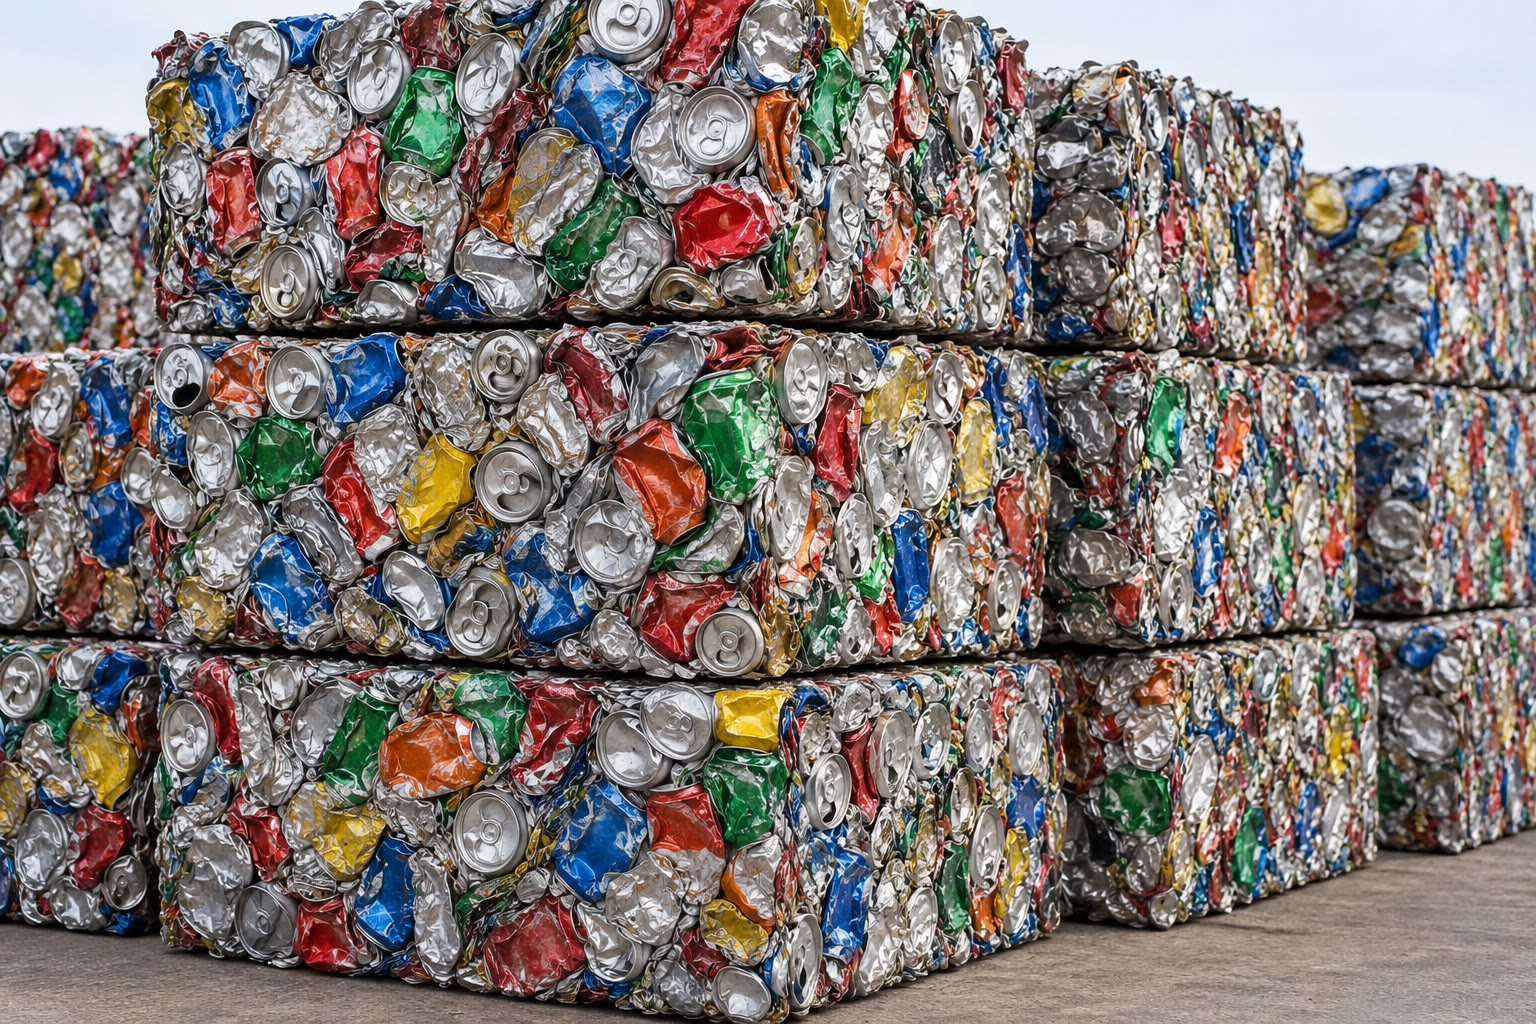
\includegraphics[width=\linewidth,height=4.6cm,keepaspectratio]{images/book1/ai/g5-can-bales.jpg}

{\small Balas de latas de aluminio aplastadas.}
\end{minipage}
\end{omfigure}

\section{Residuos y recursos}

\begin{definition}[Recurso]\label{def:g5:raw-materials-and-recycling:resource}
Un \emph{recurso}\index{recurso} es cualquier cosa que se toma de la
naturaleza y que las personas usan: el agua, la madera, las \omterm{def:g5:raw-materials-and-recycling:raw-material}{menas}, el
petróleo, la arena. Un \emph{recurso
renovable}\index{recurso renovable} vuelve a crecer o se regenera por sí
solo en el tiempo de una vida humana, como la madera de un bosque que se
replanta o la lana de las ovejas. Las \omterm{def:g5:raw-materials-and-recycling:raw-material}{menas} y el petróleo no son
renovables: una vez extraídos y usados, se acaban.
\end{definition}

\begin{proposition}[Reducir, reutilizar, reciclar]\label{prop:g5:raw-materials-and-recycling:three}
Para que los \omterm{def:g5:raw-materials-and-recycling:resource}{recursos} duren, las personas pueden, por este orden:
\begin{enumerate}
  \item \textbf{reducir}: usar menos objetos, por ejemplo menos
        envoltorios;
  \item \textbf{reutilizar}: volver a usar el mismo objeto, como un
        tarro de vidrio que se rellena o una bolsa que se vuelve a
        llevar a la tienda;
  \item \textbf{reciclar}: convertir el material en un objeto nuevo.
\end{enumerate}
Reciclar va en último lugar porque sigue necesitando energía y
máquinas; el mejor residuo es el que nunca se produce.
\end{proposition}

\section{Ejercicios}

\begin{exercise}[$\star$]\label{exo:g5:raw-materials-and-recycling:1}
¿Natural o elaborado? Madera, vidrio, lana, acero, plástico, piedra.
\end{exercise}

\begin{exercise}[$\star$]\label{exo:g5:raw-materials-and-recycling:2}
Da la \omterm{def:g5:raw-materials-and-recycling:raw-material}{materia prima} de: una hoja de papel, un tarro de vidrio, una
camiseta de algodón, una botella de plástico.
\end{exercise}

\begin{exercise}[$\star$]\label{exo:g5:raw-materials-and-recycling:3}
¿Qué es una \omterm{def:g5:raw-materials-and-recycling:raw-material}{mena}? Nombra la \omterm{def:g5:raw-materials-and-recycling:raw-material}{mena} del aluminio.
\end{exercise}

\begin{exercise}[$\star$]\label{exo:g5:raw-materials-and-recycling:4}
¿En qué contenedor tiras: un tarro de mermelada vacío, un periódico, una
lata de refresco, una botella de agua de plástico?
\end{exercise}

\begin{exercise}[$\star$]\label{exo:g5:raw-materials-and-recycling:5}
Mira la figura de la vida de un material. ¿Qué sustituye el bucle
naranja?
\end{exercise}

\begin{exercise}[$\star$]\label{exo:g5:raw-materials-and-recycling:6}
¿Renovable o no: la madera, el petróleo, la lana, la \omterm{def:g5:raw-materials-and-recycling:raw-material}{mena} de hierro, el
algodón?
\end{exercise}

\begin{exercise}[$\star$]\label{exo:g5:raw-materials-and-recycling:7}
¿Por qué el vidrio no se puede convertir otra vez en arena enfriándolo?
\end{exercise}

\begin{exercise}[$\star$]\label{exo:g5:raw-materials-and-recycling:8}
Da una manera de reducir, una de reutilizar y una de reciclar.
\end{exercise}

\begin{exercise}[$\star$]\label{exo:g5:raw-materials-and-recycling:9}
¿Por qué un contenedor de vidrio solo debe contener vidrio?
\end{exercise}

\begin{exercise}[$\star\star$]\label{exo:g5:raw-materials-and-recycling:10}
Fabricar aluminio a partir de latas viejas requiere más o menos una
veinteava parte de la energía necesaria para fabricarlo a partir de
bauxita. Una fábrica gasta 20 unidades de energía para fabricar un lote
de aluminio a partir de bauxita. ¿Cuántas unidades, más o menos,
gastaría para fabricar el mismo lote a partir de latas viejas?
\end{exercise}

\begin{exercise}[$\star\star$]\label{exo:g5:raw-materials-and-recycling:11}
¿Por qué ``reducir'' va antes que ``reciclar''?
\end{exercise}
